% book example for classicthesis.sty
\documentclass[
  oneside,
  12pt, a4paper,
  footinclude=true,
  headinclude=true,
  cleardoublepage=empty
]{scrbook}

\usepackage[linedheaders,parts,pdfspacing]{classicthesis}
\usepackage{mathtools, amsmath,amsfonts,amssymb, amsthm}
\usepackage{acronym}
\usepackage{geometry}
\usepackage{hyperref}
\usepackage[backend=bibtex,style=verbose-trad2]{biblatex}
\usepackage{float}
\usepackage{graphicx}
\usepackage{xargs}
\usepackage[colorinlistoftodos,prependcaption,textsize=tiny]{todonotes}
\newcommandx{\unsure}[2][1=]{\todo[linecolor=red,backgroundcolor=red!25,bordercolor=red,inline]{#2}}

\graphicspath{ {Figures/} }

\usepackage{tikz}
\usetikzlibrary{shapes,arrows}
\bibliography{refs}

\theoremstyle{definition}
\newtheorem{definition}{Definition}[section]

\theoremstyle{remark}
\newtheorem*{remark}{Remark}


\title{A decision support system for forecasting and optimal procurement}
\author{Neven Miculnic}

\begin{document}

\maketitle

% !TEX root = ../main.tex

%*******************************************************
% Abstract
%*******************************************************
\begin{abstract}
Optimal procurement in most industries involves forecasting of two
quantities: prices of raw materials and customer's demand.  The aim of
this work is to integrate forecasts into production planning models,
with the aim of minimizing overall procurement, holding and production
costs under demand satisfaction constraints.  The decision support
system should allow the decision maker to integrate qualitative,
unstructured information through a simple interface, for scenario
selection and solution refinement
\end{abstract}

% !TEX root = ../main.tex

\chapter{Problem definition}
\label{chap:prob-def}
\section{introduction}

This problem is a variation of the lot sizing problem in a stochastic setting. Variation is as follows. Firstly we describe deterministic variant before extending the model to stochastic setting. We have predictions for raw material supply cost $\mathbf{s}$ at future time moment $t$. The \emph{factory} converts all bought raw materials at time $t$ and stores them in a warehouse. Number of discrete time moments under consideration is denoted by $n$.

One time moment storage costs fixed amount $h$. The  holding cost is per unit and per time period.

Each time moment, $t$, we have certain demand we need to satify, denoted as $d_t$. In case there's no products in storage to satisfy demand we allow backlogging incurring a cost denoted as $b$ per unit per day, for late orders.

Our aim is to optimize our procurement policy by choosing $x_t$, which is amount of the product we buy at time moment $t$. However we are constrained by the maximum amount raw materials , $\mathbf{x^{\text{(max)}}}$, that we can buy each day.

\section{Related Work}

\subsection{Newsvendor model}
\label{sec:Newsvendor model}

The newsvendor model~\autocite{Arrow1974} is a mathematical model resembling newsvendor stand. The problem is characterized by fixed prices and uncertain demand for a perishable product, e.g. yesterdays newspapers hold no value today. Demand for newspapers is uncertain and newsvendor must decide how many newspaper to buy for reselling.


The stock in newsvendor model is only for one day, and unlike problem presented in chapter~\ref{chap:prob-def} product is not perishable, but its cost increases in each following time step.

\subsection{Dynamic lot sizing model}
\label{sec:Dynamic lot sizing model}

Dynamic lot-size model~\autocite{Wagner2004} is generalization of the Economic Order quantity model~\autocite{Harris1990} which takes into account that demand for the product varies over time. For the planning horizon of $n$ time periods we have following data:

\begin{align*}
  d_t && \text{Demand at time period $t$} \\
  h_t && \text{Holding cost at time period $t$} \\
  K_t && \text{Setup cost at time period $t$} \\
  I_0 && \text{Initial inventory} \\
\end{align*}

and decision variable $\mathbf{x}$:
\begin{align*}
  x_t && \text{Quantity purchased at time period $t$}\\
\end{align*}

For simplicity we define inventory at time period $t$ as:

\begin{align*}
  I_t &= I_0 + \sum_{t=0}^k{x_t} - \sum_{t=0}^k{d_t}\\
\end{align*}

And we want to choose optimal $x_t$, under following constraints:

\begin{align*}
  x_t &\ge 0 \; \forall t\\
  I_t &\ge 0 \; \forall t\\
\end{align*}

And we want to minimize following objective function:
\begin{equation*}
  f = \sum_t{h_t I_t + H(x_t)K_t}
\end{equation*}

where $H$ is Heaviside step function.

\subsubsection{Dynamic lot size model in stochastic setting}
\label{sub:Dynamic lot size model in stochastic setting}

Various approaches exist to handle dynamic lot sizing model in stochastic setting. The most comprehensive analysis can be found in textbook~\autocite{tempelmeier2013stochastic}. Other approaches use rolling horizon for predicting demand quantity~\autocite{cao2013adaptive} and apply modified dynamic lot sizing model by introducing backlogging, that is allowing inventory, $I_t$ to be negative with known penalty, $b_t$ per unit per time step.
\section{Formal problem definition}
\label{sec:prob-def}

\subsection{Definitions}
\label{sub:Definitions}

Following is the deterministic problem variant, and in subsequent chapters randomness and uncertainty is embedded into problem. Notation:

\begin{align*}
    \mathbf{s} &= \begin{bmatrix}
        s_1, s_2, \dotsc, s_n
    \end{bmatrix}^\intercal && \text{Supply cost vector} \\
    \mathbf{x} &= \begin{bmatrix}
        x_1, x_2, \dotsc, x_n
    \end{bmatrix}^\intercal && \text{Procurement quantity vector} \\
    \mathbf{x^{(\max)}}  & && \text{Procurement quantity limits vector} \\
    \mathbf{x}^{(b)}  & && \text{Backlogging quantity vector} \\
    \mathbf{x}^{(h)}  & && \text{Holding quantity vector} \\
    \mathbf{d} &= \begin{bmatrix}
        d_1, d_2, \dotsc, d_n
    \end{bmatrix}^\intercal && \text{Demand random vector} \\
    b & && \text{backlogging cost} \\
    h & && \text{holding cost} \\
    n & && \text{number of time moments}
\end{align*}

\unsure{Every variable for backlogging and holding vector seems unintuitive or taken. I hope $\mathbf{x}^{(b)}$ is alright since relation to $\mathbf{x}$ is clearly highlighted}

\subsection{Variables}
\label{sub:Variables}
$\mathbf{x}$ is our decision variable, as described previously. $\mathbf{x}^{(b)}$ and $\mathbf{x}^{(h)}$ are backlogging and holding variables respectively backlogging variables respectively. For simplicity
$x^{(h)}_0$, $x^{(b)}_0$,  $x^{(h)}_n$, $x^{(b)}_n$ are equal to $0$ unless otherwise noted. This specific values are explored further in Section~\ref{sec:Variants}.

\subsection{Constraints}
\label{sub:Constraints}
\begin{align*}
    x_t &\le x^{(\max)}_t & \forall t\\
    x_t &\ge 0 & \forall t\\
    x^{(b)}_t &\ge 0 & \forall t\\
    x^{(h)}_t &\ge 0 & \forall t\\
    x_t + x^{(h)}_{t - 1} + x^{(b)}_{t} &= d_t + x^{(h)}_t + h^{(b)}_{t - 1} & \forall t \\
    x^{(h)}_0 + x^{(b)}_n + \sum_{t=1}^n{x_i} &= \sum_{t=1}^n{d_i} + x^{(b)}_0 + x^{(h)}_n &\\
\end{align*}

\section{Objective function}

\begin{definition}{$c(t)$}
defines total speeding we pay at time $t$.
    \begin{equation}
        \label{eq:cost-t}
        c(t) = s_t x_t + b x^{(b)}_t + h x^{(h)}_t
    \end{equation}
\end{definition}

\begin{definition}{$f$}
    is objective function for this problem. Our aim is to minimize it.
    \begin{equation}
        f =  \sum_t{c(t)} = \sum_t{ s_t x_t + b x^{(b)}_t + h x^{(h)}_t}
        \label{eq:cost-f}
    \end{equation}
\end{definition}

% !TEX root = ../main.tex

\chapter{Deterministic approach}
\label{chap:Deterministic approach}

\section{Modelling approaches}

Problem as defined in~\ref{chap:prob-def} can be reduced to two well known problems: transportation and min-cost max flow problem. In both cases knowning $\mathbf{x}$ implies all needed network parameters given $b, h \ge 0$.  This fact can easily be observed from flow conservation on intermediate nodes as in fig~\ref{fig:mcmf-model}. They need to have net flow 0, and with their $x_t$ and $d_t$ determined, only thing left is determining $\mathbf{x_b}$ and $\mathbf{x_h}$, which can be uniquely defined since in optimal placement at same time moment one of them must be zero (since it's suboptimal to hold product and pay backlogging cost when product is in stock).

\subsection{Transportation problem reduction}
\label{subs:Transportation problem reduction}

For transportation problem reduction we need cost matrix for satisfying demand at $j$ with supply at time moment $i$. It is given as follows:

\begin{definition}{$\mathbf{C}$}
matrix defines cost for satisfying demand with specific raw supply material purchase date. It's element $c_{ij}$ equals:

\begin{equation*}
    c_{ij} = \begin{cases}
        b \left( i - j \right) + s_i & j < i \\
        h \left( j - i \right) + s_i & j \ge i
    \end{cases}
\end{equation*}
That is using purchases raw materials at $i$ to satisfy demand at time moment $j$ incurs cost $c_{ij}$.
\end{definition}

Maximum supply $\mathbf{x_{\max}}$ is given, so is the demand vector $\mathbf{d}$. Since transportation problem required equal supply and demand nodes, we add dummy demand node sucking out excess supply.

Transportation problem \autocite{or-textbook} is easy reduction since we have cost matrix $\mathbf{C}$ defining ``transportation'' costs associated with each possible assignment option. For successful reduction we only need adding dummy source or destination as described in \autocite{or-textbook}

\subsection{Min cost max flow reduction}
\label{sub:Min cost max flow reduction}

We can exploit additional problem structure to achieve superior performance and modeling capabilities. In figure~\ref{fig:mcmf-model} we see network architecture.

\begin{figure}[h]
\label{fig:mcmf-model}
  \centering
  
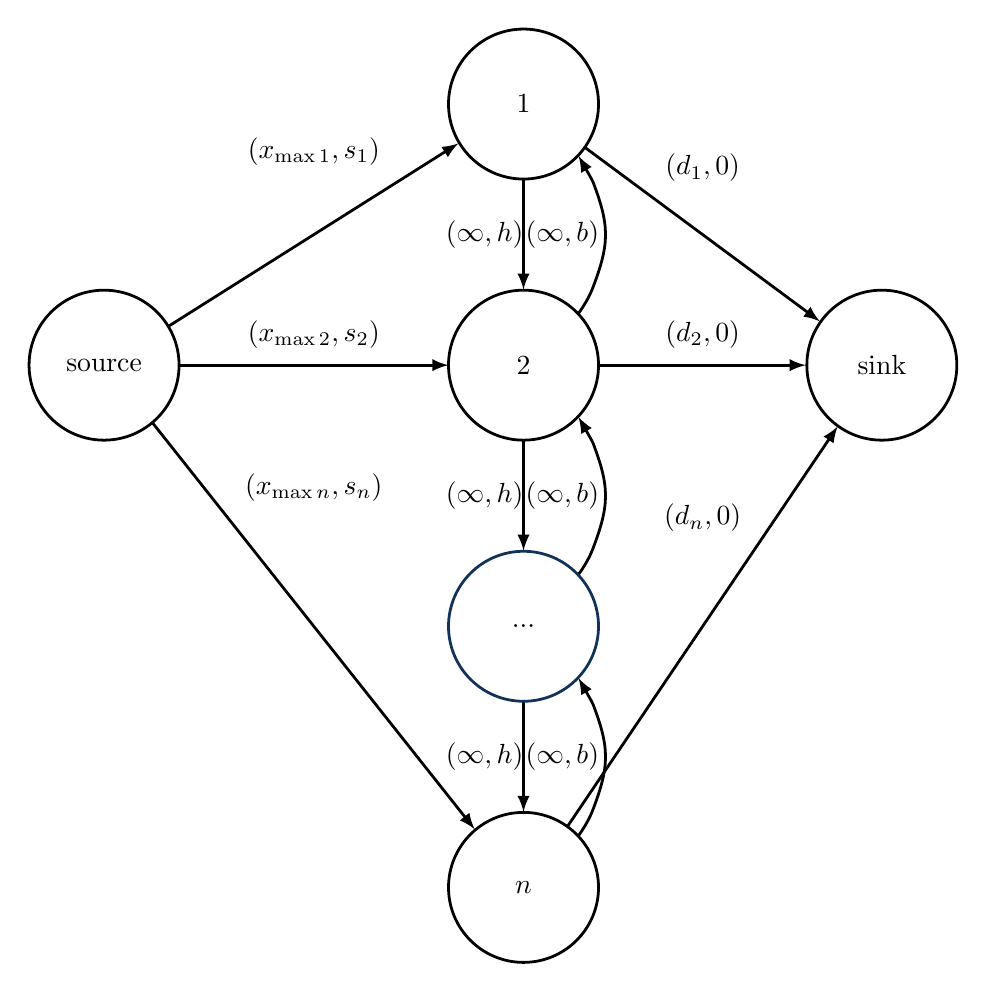
\begin{tikzpicture}[>=latex,line join=bevel,]
  \pgfsetlinewidth{1bp}
%%
\begin{scope}
  \pgfsetstrokecolor{black}
  \definecolor{strokecol}{rgb}{1.0,1.0,1.0};
  \pgfsetstrokecolor{strokecol}
  \definecolor{fillcol}{rgb}{1.0,1.0,1.0};
  \pgfsetfillcolor{fillcol}
  \filldraw (0.0bp,0.0bp) -- (0.0bp,336.0bp) -- (334.0bp,336.0bp) -- (334.0bp,0.0bp) -- cycle;
\end{scope}
\begin{scope}
  \pgfsetstrokecolor{black}
  \definecolor{strokecol}{rgb}{1.0,1.0,1.0};
  \pgfsetstrokecolor{strokecol}
  \definecolor{fillcol}{rgb}{1.0,1.0,1.0};
  \pgfsetfillcolor{fillcol}
  \filldraw (0.0bp,0.0bp) -- (0.0bp,336.0bp) -- (334.0bp,336.0bp) -- (334.0bp,0.0bp) -- cycle;
\end{scope}
  \pgfsetcolor{black}
  % Edge: n -> m
  \draw [->] (197.79bp,45.647bp) .. controls (199.91bp,48.565bp) and (201.75bp,51.712bp)  .. (203.0bp,55.0bp) .. controls (209.02bp,70.78bp) and (209.02bp,77.22bp)  .. (203.0bp,93.0bp) .. controls (202.92bp,93.205bp) and (202.84bp,93.41bp)  .. (197.79bp,102.35bp);
  \definecolor{strokecol}{rgb}{0.0,0.0,0.0};
  \pgfsetstrokecolor{strokecol}
  \draw (192.0bp,74.0bp) node {$(\infty, b)$};
  \draw (203.79bp,51.647bp) node {$$};
  \draw (203.79bp,96.353bp) node {$$};
  % Edge: m -> n
  \draw [->] (178.0bp,93.872bp) .. controls (178.0bp,84.622bp) and (178.0bp,74.113bp)  .. (178.0bp,54.189bp);
  \draw (164.0bp,74.0bp) node {$(\infty, h)$};
  \draw (184.0bp,90.872bp) node {$$};
  \draw (184.0bp,54.189bp) node {$$};
  % Edge: source -> 2
  \draw [->] (54.295bp,215.0bp) .. controls (78.339bp,215.0bp) and (114.12bp,215.0bp)  .. (150.97bp,215.0bp);
  \draw (102.5bp,226.0bp) node {$(x_{\max 2}, s_2)$};
  \draw (60.295bp,209.0bp) node {$$};
  \draw (144.97bp,209.0bp) node {$$};
  % Edge: 2 -> 1
  \draw [->] (197.79bp,233.65bp) .. controls (199.91bp,236.57bp) and (201.75bp,239.71bp)  .. (203.0bp,243.0bp) .. controls (209.02bp,258.78bp) and (209.02bp,265.22bp)  .. (203.0bp,281.0bp) .. controls (202.92bp,281.21bp) and (202.84bp,281.41bp)  .. (197.79bp,290.35bp);
  \draw (192.0bp,262.0bp) node {$(\infty, b)$};
  \draw (203.79bp,239.65bp) node {$$};
  \draw (191.79bp,284.35bp) node {$$};
  % Edge: n -> sink
  \draw [->] (193.82bp,48.934bp) .. controls (216.41bp,82.381bp) and (259.56bp,146.25bp)  .. (291.08bp,192.92bp);
  \draw (242.5bp,160.0bp) node {$(d_n, 0)$};
  \draw (187.82bp,42.934bp) node {$$};
  \draw (285.08bp,186.92bp) node {$$};
  % Edge: m -> 2
  \draw [->] (197.79bp,139.65bp) .. controls (199.91bp,142.57bp) and (201.75bp,145.71bp)  .. (203.0bp,149.0bp) .. controls (209.02bp,164.78bp) and (209.02bp,171.22bp)  .. (203.0bp,187.0bp) .. controls (202.92bp,187.21bp) and (202.84bp,187.41bp)  .. (197.79bp,196.35bp);
  \draw (192.0bp,168.0bp) node {$(\infty, b)$};
  \draw (203.79bp,145.65bp) node {$$};
  \draw (203.79bp,190.35bp) node {$$};
  % Edge: 2 -> m
  \draw [->] (178.0bp,187.87bp) .. controls (178.0bp,178.62bp) and (178.0bp,168.11bp)  .. (178.0bp,148.19bp);
  \draw (164.0bp,168.0bp) node {$(\infty, h)$};
  \draw (184.0bp,184.87bp) node {$$};
  \draw (184.0bp,148.19bp) node {$$};
  % Edge: 1 -> sink
  \draw [->] (200.26bp,293.27bp) .. controls (221.14bp,277.81bp) and (253.17bp,254.1bp)  .. (284.67bp,230.78bp);
  \draw (242.5bp,286.0bp) node {$(d_1, 0)$};
  \draw (206.26bp,287.27bp) node {$$};
  \draw (278.67bp,224.78bp) node {$$};
  % Edge: 1 -> 2
  \draw [->] (178.0bp,281.87bp) .. controls (178.0bp,272.62bp) and (178.0bp,262.11bp)  .. (178.0bp,242.19bp);
  \draw (164.0bp,262.0bp) node {$(\infty, h)$};
  \draw (184.0bp,281.87bp) node {$$};
  \draw (184.0bp,245.19bp) node {$$};
  % Edge: source -> n
  \draw [->] (44.515bp,194.16bp) .. controls (71.142bp,160.57bp) and (123.63bp,94.338bp)  .. (160.41bp,47.931bp);
  \draw (102.5bp,171.0bp) node {$(x_{\max n}, s_n)$};
  \draw (50.515bp,188.16bp) node {$$};
  \draw (154.41bp,53.931bp) node {$$};
  % Edge: source -> 1
  \draw [->] (50.307bp,229.07bp) .. controls (75.653bp,245.06bp) and (117.2bp,271.27bp)  .. (154.54bp,294.83bp);
  \draw (102.5bp,292.0bp) node {$(x_{\max 1}, s_1)$};
  \draw (56.307bp,223.07bp) node {$$};
  \draw (148.54bp,288.83bp) node {$$};
  % Edge: 2 -> sink
  \draw [->] (205.01bp,215.0bp) .. controls (223.63bp,215.0bp) and (248.96bp,215.0bp)  .. (279.59bp,215.0bp);
  \draw (242.5bp,226.0bp) node {$(d_2, 0)$};
  \draw (211.01bp,209.0bp) node {$$};
  \draw (273.59bp,209.0bp) node {$$};
  % Node: m
\begin{scope}
  \definecolor{strokecol}{rgb}{0.07,0.2,0.34};
  \pgfsetstrokecolor{strokecol}
  \draw (178.0bp,121.0bp) ellipse (27.0bp and 27.0bp);
  \definecolor{strokecol}{rgb}{0.0,0.0,0.0};
  \pgfsetstrokecolor{strokecol}
  \draw (178.0bp,121.0bp) node {$...$};
\end{scope}
  % Node: n
\begin{scope}
  \definecolor{strokecol}{rgb}{0.0,0.0,0.0};
  \pgfsetstrokecolor{strokecol}
  \draw (178.0bp,27.0bp) ellipse (27.0bp and 27.0bp);
  \draw (178.0bp,27.0bp) node {$n$};
\end{scope}
  % Node: 1
\begin{scope}
  \definecolor{strokecol}{rgb}{0.0,0.0,0.0};
  \pgfsetstrokecolor{strokecol}
  \draw (178.0bp,309.0bp) ellipse (27.0bp and 27.0bp);
  \draw (178.0bp,309.0bp) node {$1$};
\end{scope}
  % Node: source
\begin{scope}
  \definecolor{strokecol}{rgb}{0.0,0.0,0.0};
  \pgfsetstrokecolor{strokecol}
  \draw (27.0bp,215.0bp) ellipse (27.0bp and 27.0bp);
  \draw (27.0bp,215.0bp) node {source};
\end{scope}
  % Node: 2
\begin{scope}
  \definecolor{strokecol}{rgb}{0.0,0.0,0.0};
  \pgfsetstrokecolor{strokecol}
  \draw (178.0bp,215.0bp) ellipse (27.0bp and 27.0bp);
  \draw (178.0bp,215.0bp) node {$2$};
\end{scope}
  % Node: sink
\begin{scope}
  \definecolor{strokecol}{rgb}{0.0,0.0,0.0};
  \pgfsetstrokecolor{strokecol}
  \draw (307.0bp,215.0bp) ellipse (27.0bp and 27.0bp);
  \draw (307.0bp,215.0bp) node {sink};
\end{scope}
%
\end{tikzpicture}


  \caption{min cost max flow model. Arcs are labeled (capacity, cost)}
\end{figure}

\subsection{Feasible solution heuristic}
\label{subs:Feasible solution heuristic}
Since this problem has special structure, not found in original transportation problem, this heuristic enables us to construct better initial feasible solution. We can solve relaxed problem where backlogging is forbidden in $\mathcal{O}(n \log{} n)$ using greedy approach:

\begin{verbatim}
    For each $d_i$ in order from 1 to $n$ do:
        While $d_i$ not satisfied:
            Find cheapest $x_k$ positive supply node and
            satisfy as much as possible
\end{verbatim}

By the end of this procedure we're going to satisfy all demand in optimal way in case it's possible to to do. Naive implementation results in $\mathcal{O}(n^2)$ runtime, however we can use priority queue, with heap backing implementation for $\mathcal{O}(n\log{}n)$ runtime.

This priority queue is sorted by costs and since all costs raise by constant amount between $d_i$ and $d_{i+1}$ we can keep it updated in $\mathcal{O}(1)$.

\section{Variants}
\label{sec:Variants}

Problem as defined previously could seem rather simplistic and not allowing useful extensions users might want, such as current storage amount and similar. In following few subsections most useful extensions are described.

\subsection{Starting storage capacity}
in case we have already certain number of product in stock we can easily embed that knowledge into model by adding new supplier/node as new decision variable $x_0$. It's maximum, $x_{\max0}$ is equal to starting storage capacity, and $c_{0j} = \left( j - 1 \right) h$

\subsection{Ending storage requirement}
\label{subs:Ending storage requirement}
For example we'd like to have some extra product in stock by the end of analysis, and it's quite easy to accommodate such requirement. Simple add to $d_n$ ending storage requirement, thus obtaining new $d_n$.

\subsection{Time Shifted ordering}
\label{subs:Time Shifted ordering}
If we order raw materials at $t$ they might arrive at later time moment $t+\Delta_t$. This can easily be modeled via variable substitution. For different $\Delta_t$ depending on the $t$ or multiple suppliers see Subsection~\ref{subs:Multiple raw material suppliers}

\subsection{Multiple raw material suppliers}
\label{subs:Multiple raw material suppliers}
Adding new raw material suppliers with different costs cannot be done as per original model specification, however reduction to presented problems is straightforward.

\subsection{Allowing future backlogging}
\label{subs:Allowing future backlogging}
In model as described, time stops at time moment $n$, however, in realistic scenario we're looking at only short time snapshot of ongoing process. To allow such future purchases to backlog at previous times, we can extend the model with $m$ future moments:
\begin{align*}
    d_{n+i} &= 0  && \\
    x_{\max{n+i}} &= y_i  && \text{allowable backlogging from future supply purchases}\\
    \mathbf{C}  & && \text{as previously defined, simply extended} \\
    \mathbf{s} &&& \text{extended with future costs}
\end{align*}
for $i$ in $1, 2, \dotsc, m$

% !TEX root = ../main.tex

\chapter{Introducing randomness}
\label{chap:solution-randomness}

\unsure{This whole chapter is in rewriting.}

TODO: This is very much work in progress since I have no idea whether am I taking the right approach.

... fill this in

First we are going to analise problem deeply without presuming any independence or probability distribution on random variables. Later in subsequent chapters we are going to focus more on where demand at time $t$ has independent Gaussian distribution and mean.

\section{Cost function}
\begin{align*}
\shortintertext{The minimizing function is:}
    & \operatorname{E} \left[
        \mathbf{s}^\intercal\mathbf{x} + \sum{c(t)}
    \right] \\
\shortintertext{Due to linerality of expectation and $x$ being variable it's equal to:}
    & \mathbf{x} \operatorname{E} \left[
        \mathbf{s}^\intercal
        \right] +
        \operatorname{E} \left[ \sum{c(t)} \right] \\
\end{align*}

Therefore only needed modeling information for supply cost is its expectation $\operatorname{E} \left[ \mathbf{s} \right]$. The other part is more trickier since $D_i$ and $D_j$ aren't usually independent.

\section{Handling demand cost non-linearity}
\label{sec:Handling demand cost non-linearity}

As we can see in equation~\ref{eq:cost-t} we have non-linearity depending whether we're satifying all demand or are we backlogging demand at time $t$. Therefore here are two possible solutions for minimizing objective function~\ref{eq:cost-f}.

\subsubsection{Simulation}
\label{subs:Simulation}

We generate multiple scenarios for demand vector, $d$ according to probability distribution. For small $n$ and relatively small number of outcomes in each random variable we can exhaustedly model each scenario, scale it appropriately and feed to MIP solver\footnote{There's a trick on using binary variable for discontinuity in cost function~\ref{eq:cost-t}}

\subsubsection{Safety net approach}
\label{subs:Safety net approach}

Alternatively, we can artificially add new constraints and avoiding backlogging with arbitrary probably. This model assumes backlogging cost are significantly greater than storage cost, that is backlogging penalty is severe.

Thus we chose values arbitrary realizations of random variables $D_t$ and add additional constraints of the form:

\begin{equation}
    \label{eq:new-cost-t}
    X_t \ge D_i \; \forall t
\end{equation}

which reduces cost function~\ref{eq:cost-t} to:
\[
c(t) = h \left( X_i - D_i \right) \; X_i \ge D_i
\]

and enables are faster solving approaches. Given parameters $D_i$ chosen and their underlying distribution we derive non-increasing function $p(t)$ which represent probability of not breaking newly introduced constraints~\ref{eq:new-cost-t}

\subsubsection{Min-cost max flow with uncertaintiy}
\label{subs:Min-cost max flow with uncertaintiy}

Since deterministic case can be modeled with min-cost max flow, we can investigate further in this directi

\subsubsection{Stochastic Dynamic Programmnig}
\label{subs:SDP}

TODO.. maybe, I've got recommendation by a friend, need to read some papers.

% !TEX root = ../main.tex

\chapter{Application on historical dataset}
\label{chap:Application on historical dataset}

For purpose of demonstrating for demand I'm using data from US electricity consumption found~\autocite{us-elec} It offers per month aggregation of electrical utilities per state, and for purpose of illustration I'm using whole US aggregated. Data ranges from 1990 till February 2016. I'm using restricted version from 1990 till 2005 aggregated on yearly basis. Full data plot is in figure~\ref{fig:supply}

\begin{figure}[]
  \centering
  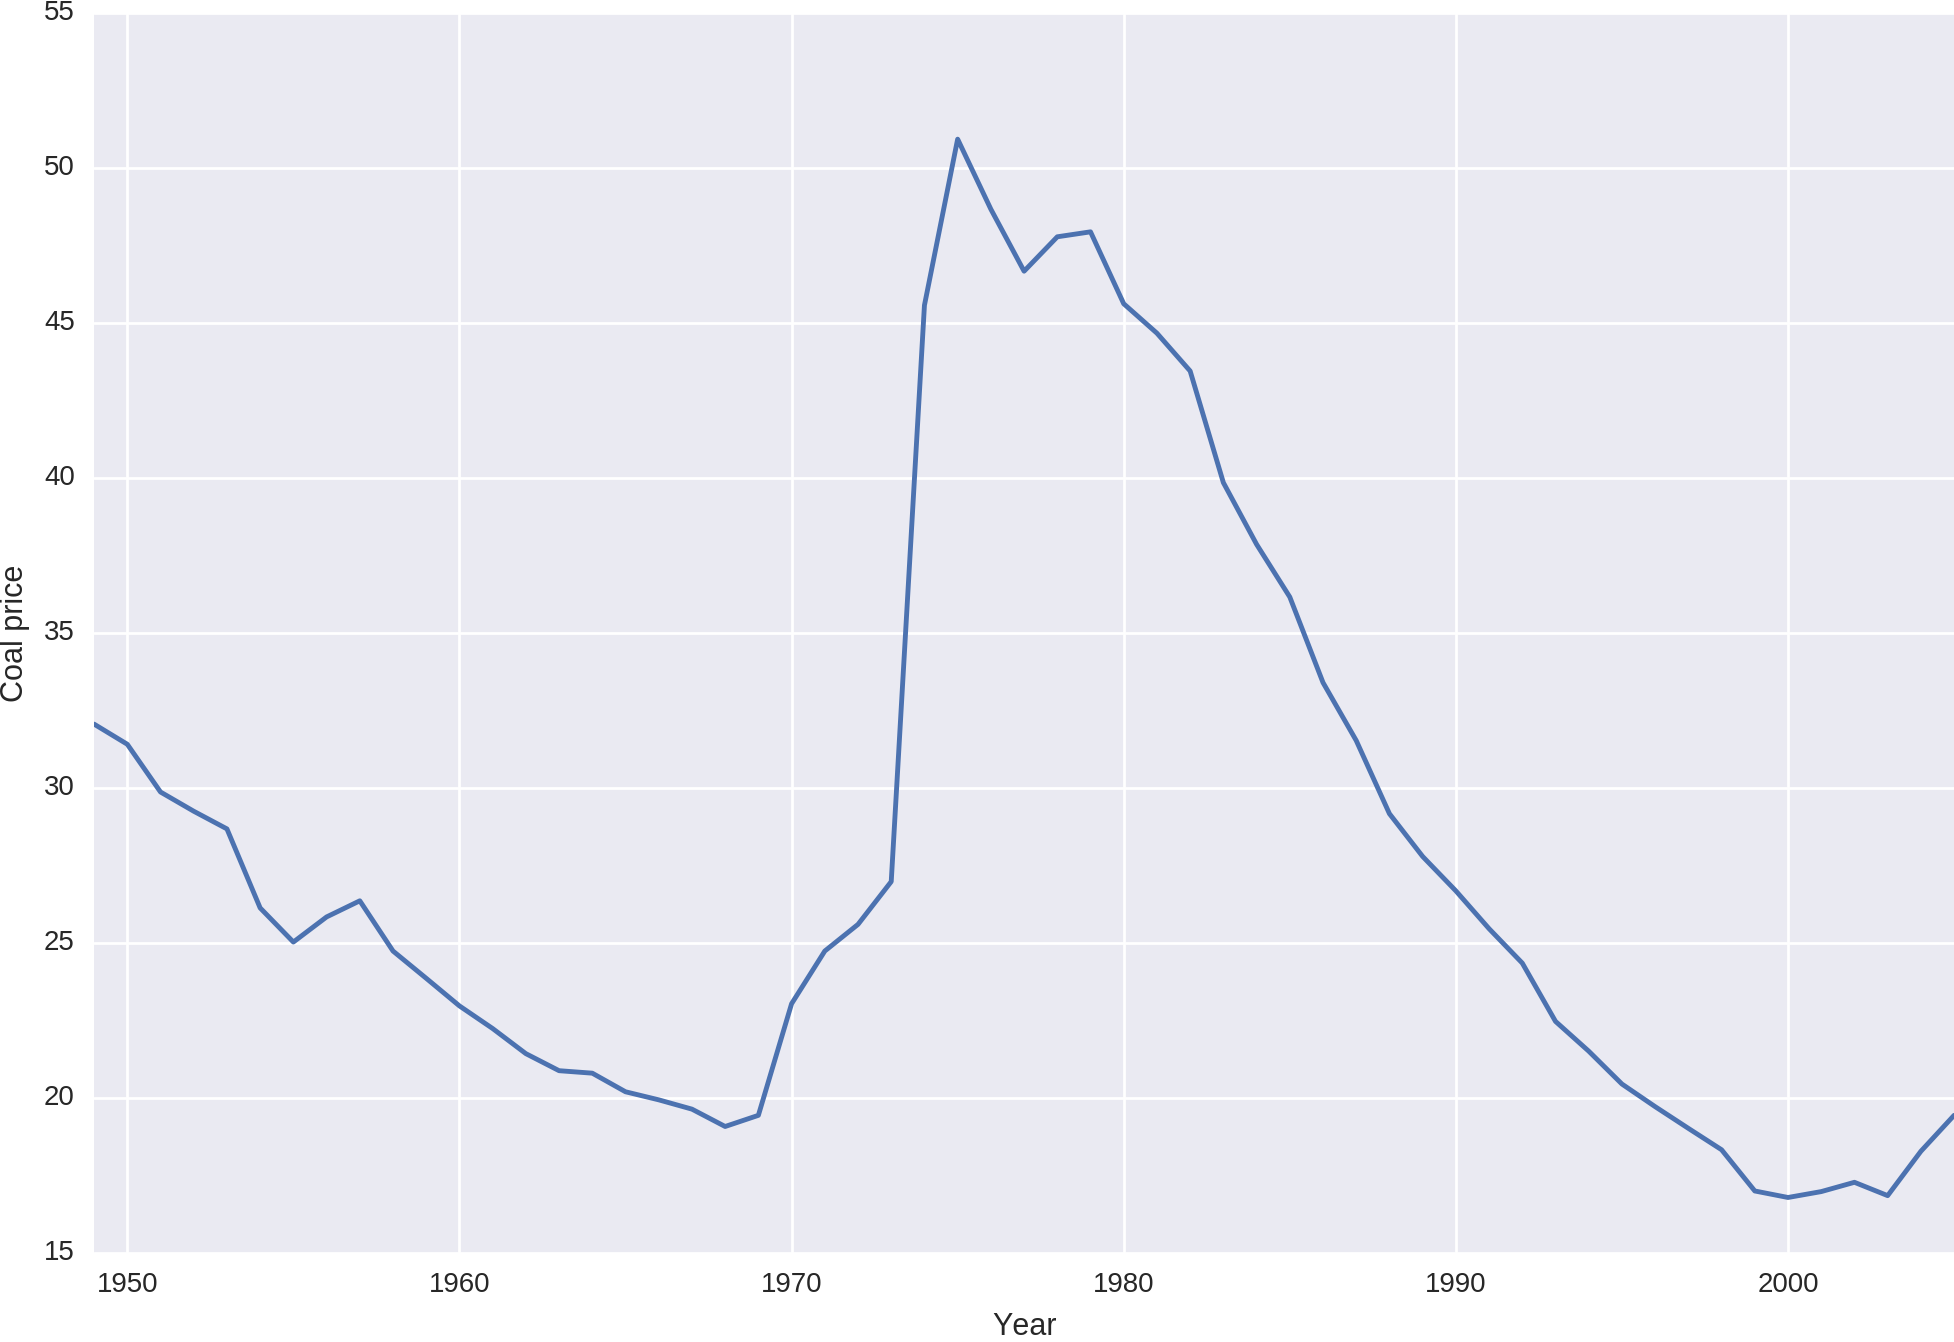
\includegraphics[width=\linewidth]{supply}
  \caption{Yearly coal prices}
  \label{fig:supply}
\end{figure}

For supply unit cost, for illustrative purposes I'm using historic American coal Price found at \autocite{us-coal}. It is yearly based from 1950 till 2005. The data is plot is in figure~\ref{fig:demand}.

For purposes of this analysis, data from 2000 till 2005 is going to be forecasted as described in previous chapter, and then compared to ideal, perfect knowledge scenario. Analysis will be conducted for various values of $\mathbf{x_{\max}}$, $b$ and $d$ model parameters.

\begin{figure}[]
  \centering
  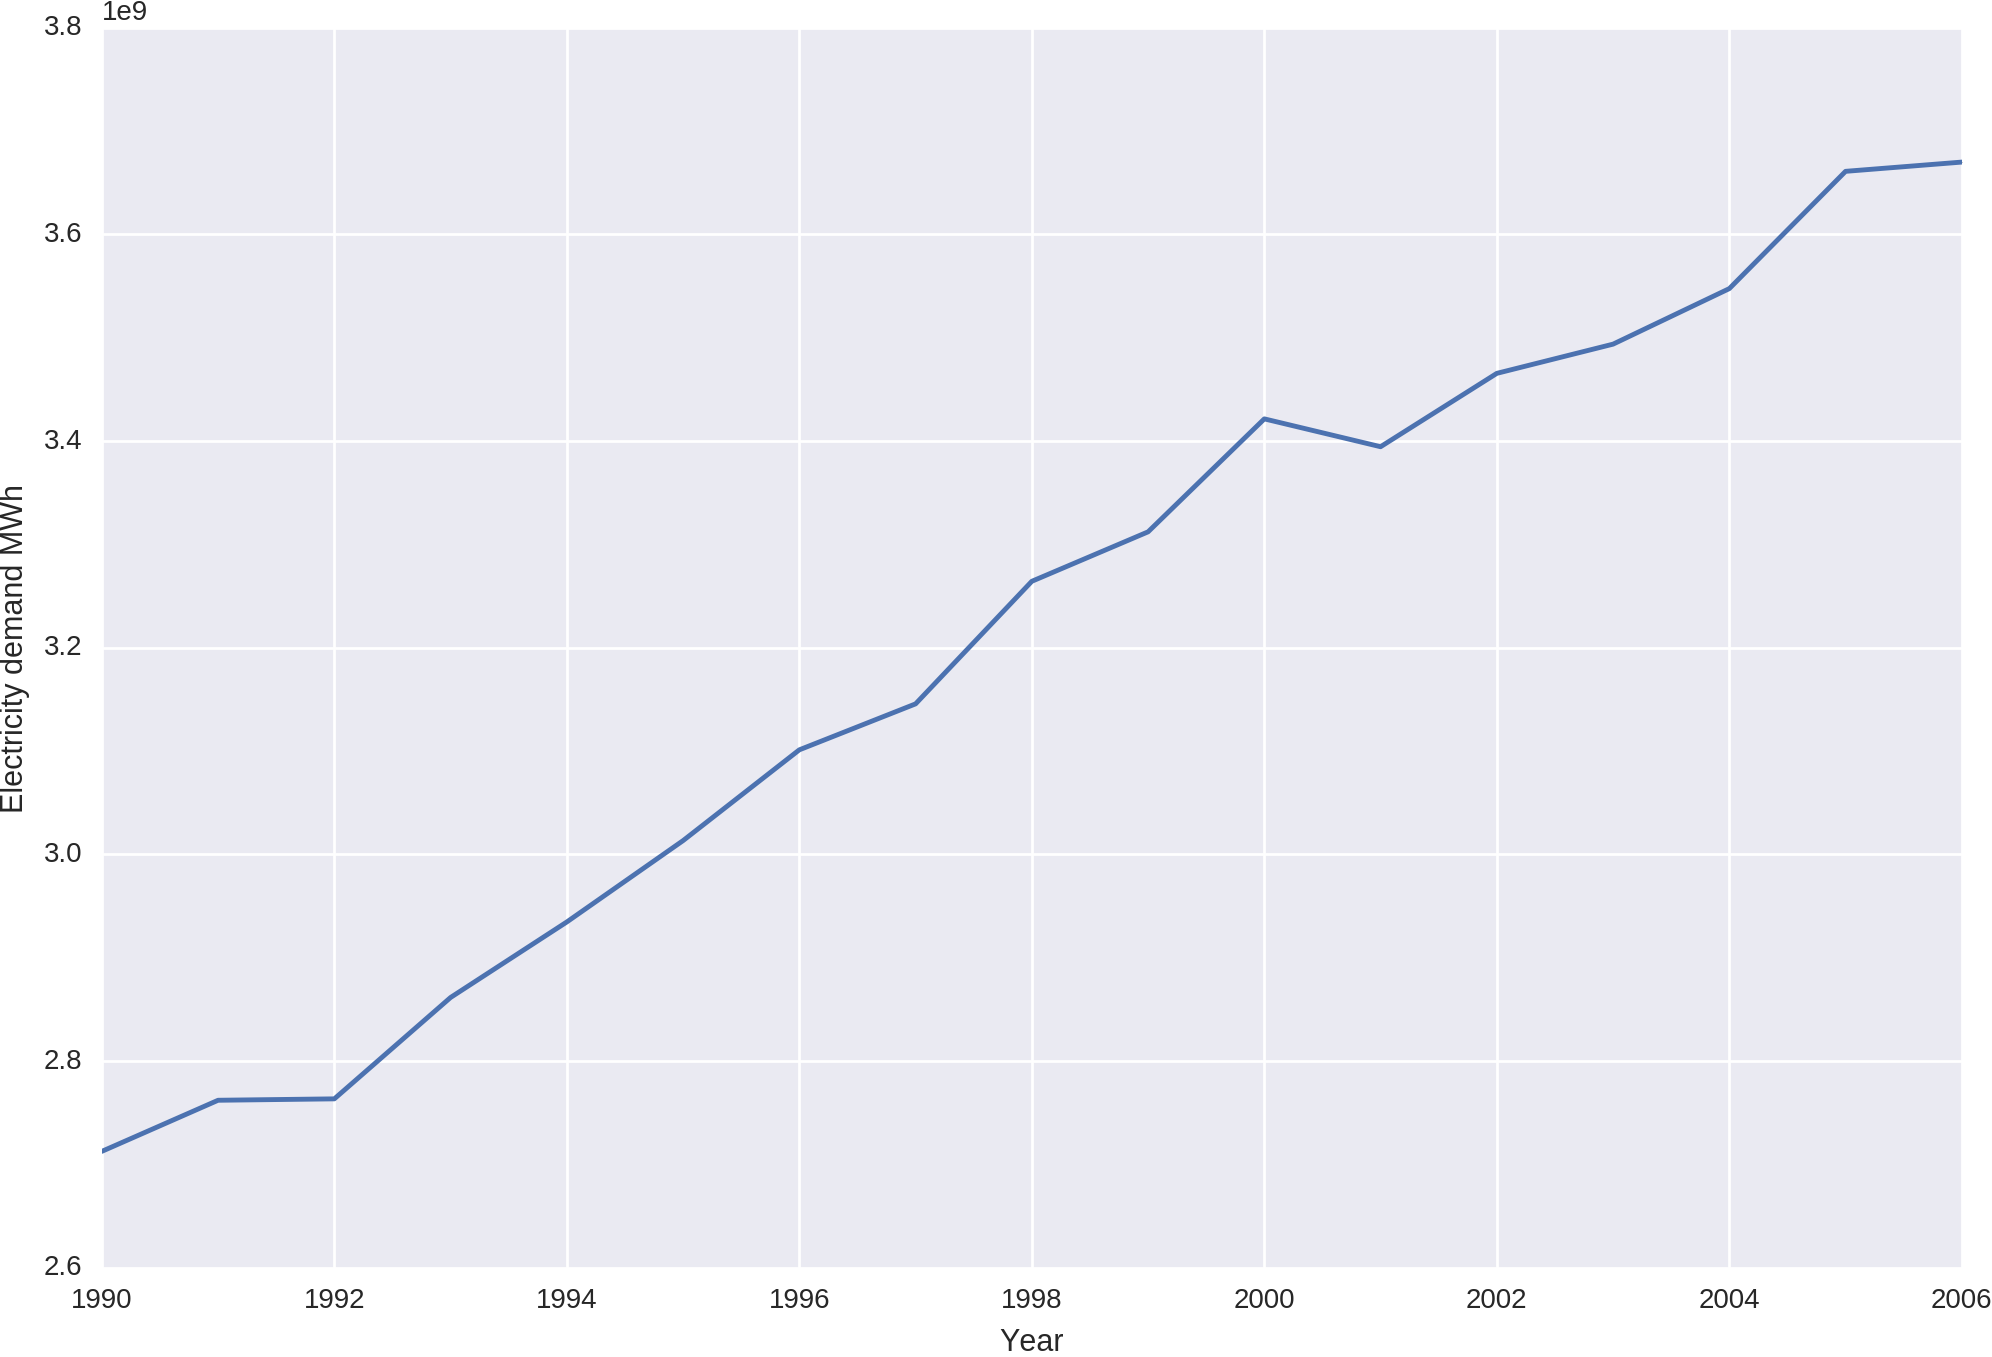
\includegraphics[width=\linewidth]{demand}
  \caption{Yearly electricity demand}
  \label{fig:demand}
\end{figure}


\printbibliography
\end{document}
